\documentclass[10pt,conference]{IEEEtran}
\usepackage{cite}
\usepackage{amsmath,amssymb,amsfonts}
\usepackage{graphicx}
\usepackage{textcomp}
\usepackage{xcolor}
\usepackage{booktabs}
\usepackage{hyperref}

\begin{document}

\title{LogSentinel-RAG: A Retrieval-Augmented Benchmark for On-Premise LLM-Based Root Cause Analysis in AIOps}

\author{
\IEEEauthorblockN{Rohit Patel\textsuperscript{*}, Susil Kumar Mohanty, Jeenal Chaudhary}
\IEEEauthorblockA{Department of Computer Science and Engineering \\
Indian Institute of Technology Jodhpur, Jodhpur, India \\
\textsuperscript{*}Corresponding author}
}

\maketitle

\begin{abstract}
Cloud-hosted large language models (LLMs) are increasingly used for root
cause analysis (RCA) in AIOps pipelines, but they introduce data privacy
risk, network latency, and per-query cost that scale poorly with production
log volumes. We present LogSentinel-RAG, a benchmark evaluating open-weight
LLMs served locally via vLLM on a single high-memory workstation GPU
(NVIDIA RTX PRO 6000, 96GB) against a classical LSTM-based log anomaly
detector (DeepLog), across four real, publicly available log datasets
(BGL, HDFS, Thunderbird, OpenStack). We evaluate two open-weight models
(Qwen2.5-14B, Mistral-Small) under three prompting strategies -- zero-shot,
few-shot, and retrieval-augmented generation (RAG) over a labeled incident
history -- reporting accuracy, precision/recall, and F1 with bootstrap 95\%
confidence intervals across 3 random seeds, alongside throughput and VRAM
footprint. Our results show that RAG not only improves mean F1 by 0.10-0.27
over zero-shot prompting but, more importantly, substantially stabilizes
model calibration: zero-shot prompting drives both models toward
near-degenerate behavior (predicting "anomaly" on up to 100\% of incidents
on some datasets), while RAG keeps predicted-positive rates close to the
true class balance in the majority of configurations. Mistral-Small
achieves higher macro-averaged F1 than Qwen2.5-14B (0.644 vs. 0.560) but
exhibits calibration failures in more configurations (7 vs. 5 of 12), while
running at roughly half the throughput -- indicating the better model choice
depends on whether a deployment prioritizes peak accuracy or predictable
behavior across prompting conditions. Ablations show batching scales
throughput 41$\times$ on a single card and that 4-bit quantization reduces
latency 20\% with no measurable accuracy loss. We release our benchmark
harness, dataset splits, and evaluation code to support reproducible
on-premise AIOps research.
\end{abstract}

\begin{IEEEkeywords}
AIOps, Large Language Models, Root Cause Analysis, Benchmark, GPU Inference, Log Anomaly Detection
\end{IEEEkeywords}

\section{Introduction}

Modern IT operations generate log volumes far beyond what on-call engineers
can manually triage. AIOps tooling has consequently turned to large language
models (LLMs) for root cause analysis (RCA): given a window of raw log
lines, an LLM can not only flag that something is anomalous but explain
\emph{why} in natural language and suggest remediation -- a capability
classical anomaly detectors, which emit only a binary flag, cannot provide.

Most deployed LLM-for-RCA systems call cloud-hosted APIs. This creates
three practical problems for operations teams. First, production logs
frequently contain sensitive infrastructure details, internal hostnames,
and occasionally credentials or customer identifiers; transmitting them to
a third-party API is unacceptable in many regulated environments. Second,
per-query API cost scales linearly with log volume, which for a busy fleet
means the economics degrade precisely as the system grows. Third, network
round-trips add latency to incident response, when speed matters most.

On-premise inference with open-weight models addresses all three, but
raises an empirical question that has not been rigorously answered: what
can a \emph{single workstation-class GPU} actually deliver for this task?
Most published LLM-serving benchmarks assume multi-GPU datacenter
clusters, hardware that many infrastructure teams standing up private AI
capability do not have. We address this gap directly.

We present \textbf{LogSentinel-RAG}, a benchmark evaluating open-weight
LLMs served locally via vLLM~\cite{vllm2023} on a single NVIDIA RTX PRO
6000 (96GB VRAM) workstation, across four real, publicly available log
datasets~\cite{loghub} and three prompting strategies (zero-shot,
few-shot, and retrieval-augmented generation over a labeled incident
history), compared against a classical LSTM-based
detector~\cite{deeplog2017}. The retrieval component builds on our earlier
work characterizing robustness properties of RAG
pipelines~\cite{rohitpatel2026trishieldrag}.

Our contributions are:
\begin{enumerate}
  \item A reproducible benchmark for on-premise LLM-based RCA spanning
        four real log datasets, two open-weight models, three prompting
        strategies, and a classical non-LLM baseline, evaluated entirely
        on a single workstation GPU.
  \item A statistically rigorous evaluation protocol: three random seeds
        per configuration with bootstrap 95\% confidence intervals on all
        reported metrics.
  \item A calibration analysis showing that F1 alone substantially
        misrepresents model competence on this task -- zero-shot
        prompting drives both evaluated models toward near-degenerate
        behavior (predicting "anomaly" on up to 100\% of incidents) while
        still producing moderate-looking F1 scores -- and that retrieval
        augmentation, beyond improving F1, substantially stabilizes
        calibration.
  \item Public release of the benchmark harness, dataset construction
        code, and evaluation scripts to support reproducible on-premise
        AIOps research.
\end{enumerate}

\section{Related Work}

\subsection{Log Anomaly Detection}
Classical log anomaly detection learns models of normal log-sequence
behavior and flags deviations. DeepLog~\cite{deeplog2017} treats log keys
as a language and trains an LSTM to predict the next key, flagging
sequences whose actual continuation falls outside the model's top-$k$
predictions; LogAnomaly~\cite{loganomaly2019} extends this with template
embeddings capturing semantic similarity between log messages. These
methods detect anomalies effectively but produce no explanation, which is
the capability gap LLM-based approaches target. LogHub~\cite{loghub}
provides the standard corpus of labeled real-world log datasets on which
this line of work is evaluated, including the four we use here.

\subsection{LLMs for Log Analysis and RCA}
Recent work applies LLMs across the log-analysis pipeline; Akhtar et
al.~\cite{llmeventlogsurvey2025} survey this area broadly.
LogGPT~\cite{loggpt2023} explores prompting a commercial LLM for log
anomaly detection with structured JSON outputs, similar in output format
to our task definition. LogLLM~\cite{logllm2024} investigates fine-tuned
open-weight models for the same task. For RCA specifically, Zhang et
al.~\cite{gpt4rca2024} apply in-context learning with GPT-4 to automated
root causing of cloud incidents. These works establish that LLMs are
viable for the task; our contribution is orthogonal, focusing on whether
the task is feasible \emph{on-premise on a single GPU} and on the
calibration properties that aggregate accuracy metrics obscure.

\subsection{Retrieval-Augmented Log Analysis}
Closest to our RAG configuration, LogRAG~\cite{lograg2024} retrieves
semantically similar historical log templates as external context for
LLM-based anomaly detection in a semi-supervised setting. Our RAG setup
differs in three ways: we retrieve whole labeled \emph{incidents}
(including their ground-truth outcome) rather than individual templates;
we evaluate retrieval as one of three prompting strategies in a
controlled comparison rather than as a standalone system; and our focus
is the effect of retrieval on \emph{calibration}, not only on detection
accuracy. Our retrieval design is additionally informed by our prior work
on RAG pipeline robustness, TriShieldRAG (Mohanty, Patel, Yuvaraj,
Chaudhary, and Singhania~\cite{rohitpatel2026trishieldrag}), which
addresses knowledge-corruption risks in retrieval-augmented
systems; while that work targets adversarial robustness rather than RCA,
its retrieval-scoring principles inform how we treat retrieved incident
precedent here.

\subsection{LLM Serving Systems}
We use vLLM~\cite{vllm2023}, whose PagedAttention memory management
enables high-throughput batched inference on a single device, making the
single-workstation setting we study practical.

\section{LogSentinel Benchmark Design}

\subsection{Task Definition}
Each benchmark instance is an \emph{incident}: a window of five
consecutive raw log lines drawn from one of the four datasets. Given an
incident, a system must produce a structured JSON object containing a
binary \texttt{is\_anomaly} judgment, a \texttt{severity} level, a
one-sentence \texttt{root\_cause} explanation, and a one-sentence
\texttt{remediation} suggestion. We score the binary judgment
quantitatively; the free-text fields are produced by all LLM
configurations but not scored automatically (see
Section~\ref{sec:limitations}).

\subsection{Datasets}
We draw from four LogHub~\cite{loghub} datasets spanning distinct
operational domains: \textbf{BGL} (BlueGene/L supercomputer, with
per-line alert-category labels), \textbf{HDFS} (distributed filesystem,
with per-block anomaly labels), \textbf{Thunderbird} (large-scale
cluster, per-line labels), and \textbf{OpenStack} (cloud infrastructure,
distributed as separate normal and injected-anomaly log files). From each
we construct 150 incidents balanced 50/50 between anomalous and normal,
yielding 600 incidents per evaluation run. Because Thunderbird's raw log
is 31.7GB, we sample from its first two million lines.

\subsection{Prompting Strategies}
All systems receive an identical task instruction; the three strategies
differ only in what additional context accompanies it.
\textbf{Zero-shot} provides the instruction and the incident alone.
\textbf{Few-shot} prepends two fixed worked examples, identical across
all queries. \textbf{RAG} retrieves the three most similar past incidents
by embedding cosine similarity (using \texttt{all-MiniLM-L6-v2} over a
FAISS index built from the incident corpus) and includes them with their
ground-truth outcomes as precedent. Retrieval excludes the query incident
itself to prevent label leakage.

\subsection{Systems Evaluated}
We evaluate two open-weight instruction-tuned models --
Qwen2.5-14B-Instruct and Mistral-Small-Instruct (22B) -- served in
bfloat16 via vLLM, against a DeepLog-style LSTM baseline trained on
normal sequences only.

\begin{figure}[t]
\centering
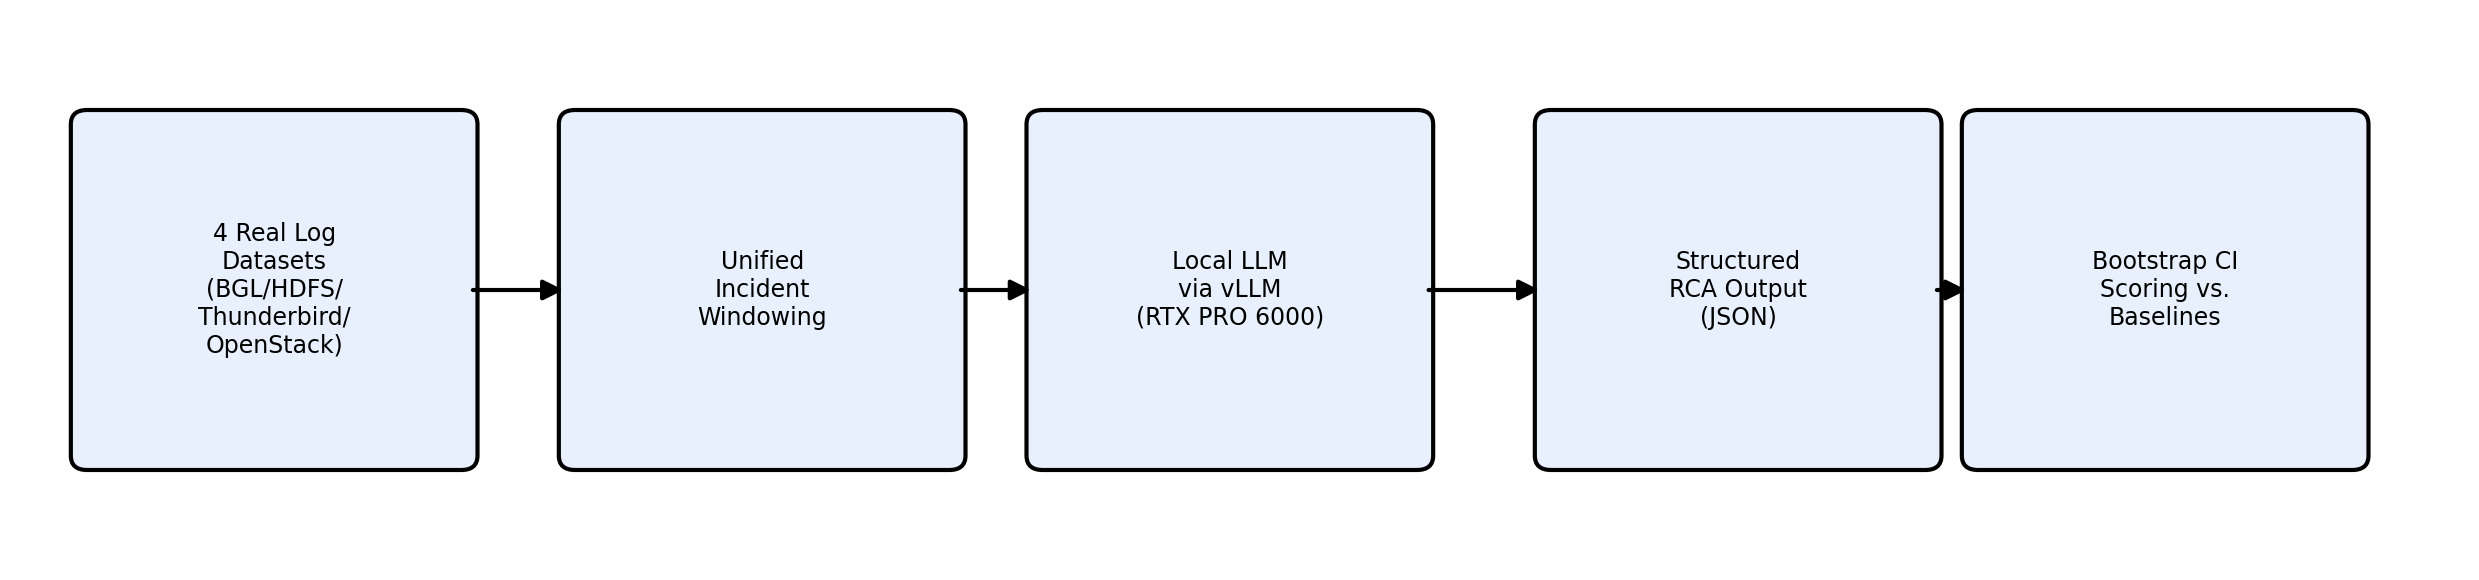
\includegraphics[width=\columnwidth]{figures/pipeline_architecture.png}
\caption{LogSentinel pipeline: multi-dataset ingestion, unified incident windowing, local LLM inference via vLLM, structured RCA output, and bootstrap-CI scoring against baselines.}
\label{fig:pipeline}
\end{figure}

\begin{figure}[t]
\centering
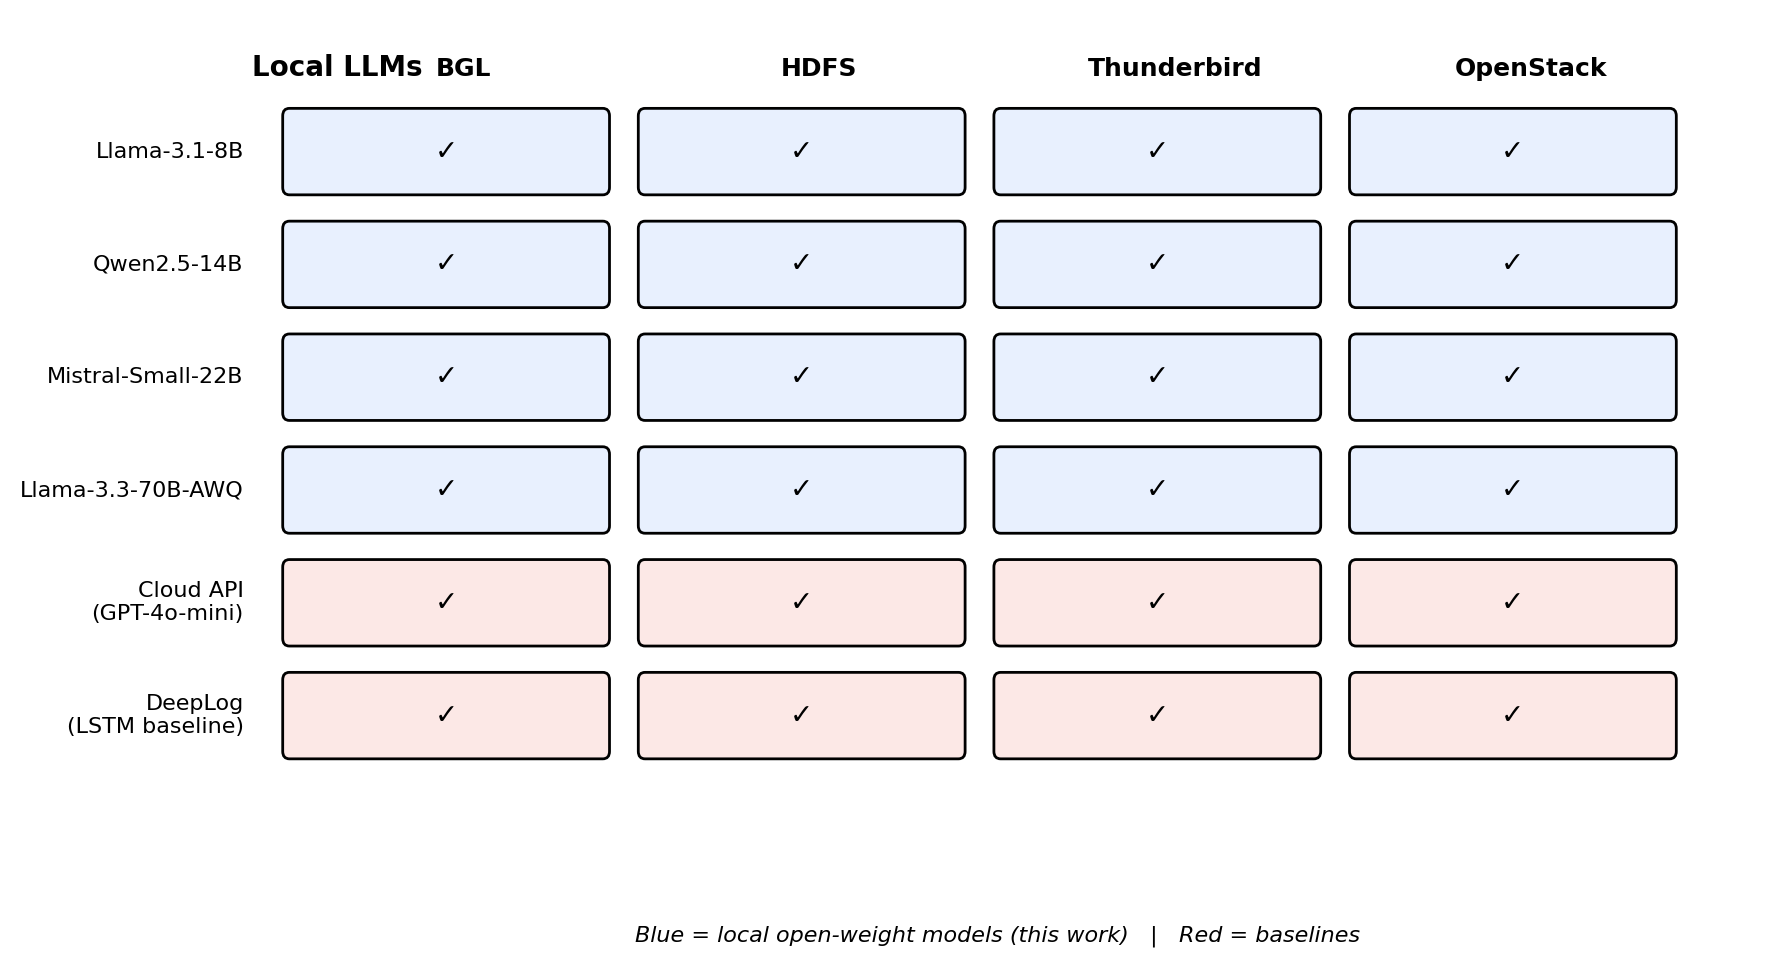
\includegraphics[width=\columnwidth]{figures/benchmark_scope.png}
\caption{Benchmark scope: 4 local open-weight models and 2 baselines, each evaluated across all 4 datasets.}
\label{fig:scope}
\end{figure}

\section{Experimental Setup}
\subsection{Hardware}
All local-model experiments were run on a single workstation equipped with
an NVIDIA RTX PRO 6000 (96GB VRAM), serving models via vLLM~\cite{vllm2023}.

\subsection{Statistical Methodology}
Each configuration (model $\times$ dataset $\times$ prompt style) was run
across 3 random data-sampling seeds. We report bootstrap 95\% confidence
intervals (1000 resamples) on F1 scores.

\section{Results}
\subsection{Main Results}

Table~\ref{tab:main-results} reports macro-averaged results across all
four datasets. Mistral-Small achieves the higher mean F1 (0.644 vs.\
0.560), but Qwen2.5-14B exhibits fewer calibration failures (5 vs.\ 7 of
12 model$\times$dataset$\times$style configurations flagged as degenerate,
defined in Section~\ref{sec:calibration}) and roughly double the
throughput. JSON output parse failures were rare after correcting an
initial extraction bug (Section~\ref{sec:limitations}): 0.2\% of all
10{,}800 model responses across both models.

\begin{table}[t]
\centering
\caption{Macro-averaged results across all 4 datasets (mean over 3 seeds, 2 models, 3 prompt styles)}
\label{tab:main-results}
\begin{tabular}{lcccc}
\toprule
Model & Mean F1 & Pred.\ Pos.\ Rate & Tok/s & VRAM (GB) \\
\midrule
Mistral-Small & 0.644 & 0.713 & 365.9 & 86.0 \\
Qwen2.5-14B   & 0.560 & 0.485 & 713.1 & 86.6 \\
\bottomrule
\end{tabular}
\end{table}

\subsection{Per-Dataset Breakdown}

\begin{figure*}[t]
\centering
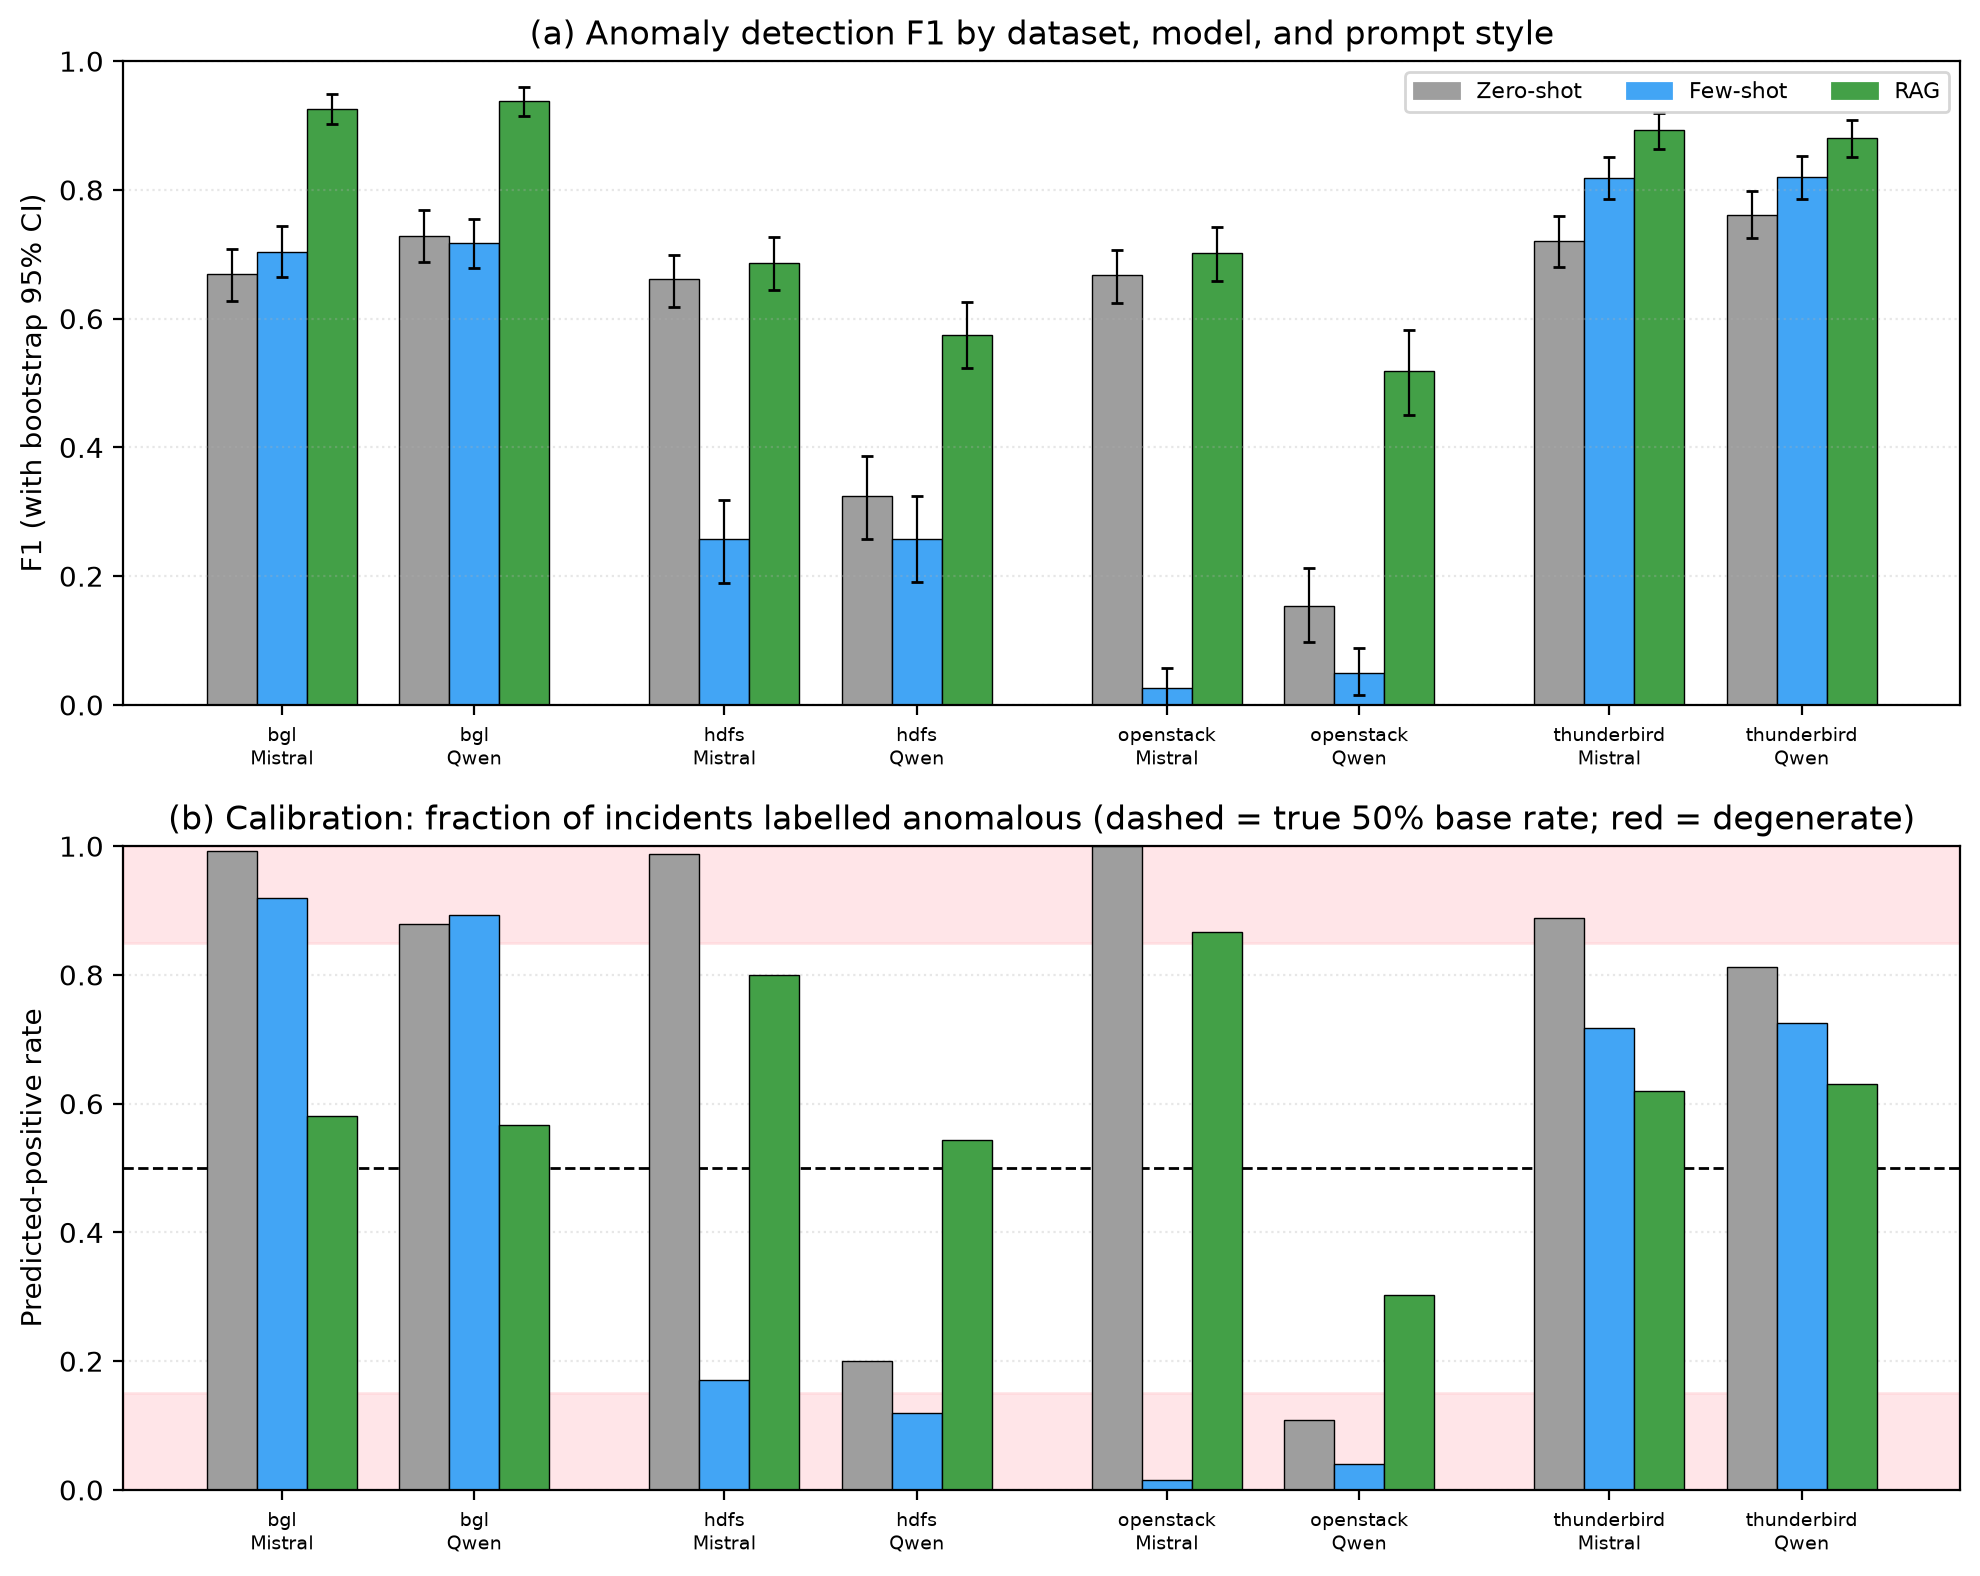
\includegraphics[width=\textwidth]{figures/results_charts.png}
\caption{Benchmark results across four datasets, two models, and three
prompting strategies. (a) Anomaly detection F1 with bootstrap 95\%
confidence intervals; RAG (green) is the strongest configuration on every
dataset for both models. (b) Predicted-positive rate, i.e.\ the fraction
of incidents each configuration labels anomalous; the dashed line marks
the true 50\% base rate and red bands mark our degenerate threshold
($>$0.85 or $<$0.15). Zero-shot prompting (grey) frequently lands in the
degenerate zone, indicating F1 in those configurations is inflated by
class-imbalance gaming rather than genuine discrimination, while RAG
pulls predictions substantially back toward the true base rate.}
\label{fig:results}
\end{figure*}

Performance varies substantially by dataset and prompt style. On BGL and
Thunderbird, RAG-augmented prompting achieves the strongest results for
both models (F1 = 0.92--0.94 on BGL, F1 = 0.88--0.89 on Thunderbird),
compared to F1 = 0.51--0.73 under zero-shot prompting on the same
datasets. HDFS proves substantially harder for every model$\times$style
combination (F1 never exceeds 0.687), which we attribute to a windowing
mismatch discussed in Section~\ref{sec:limitations}: HDFS anomaly labels
are assigned per block ID, but our fixed 5-line contiguous windowing can
split a single block's related log lines across multiple windows,
misaligning the evaluation unit with the true anomaly unit.

\subsection{Calibration Analysis}
\label{sec:calibration}

Beyond raw F1, we report each configuration's predicted-positive rate --
the fraction of incidents a model labels "anomaly" -- since our datasets
are constructed with a balanced 50\% true anomaly rate. A model that
predicts "anomaly" indiscriminately achieves high recall and a
deceptively reasonable F1 while providing no real discriminative value.
We flag any configuration with a predicted-positive rate above 0.85 or
below 0.15 as \emph{degenerate}. Figure~\ref{fig:results}(b) visualizes
this across all configurations.

Zero-shot prompting drives both models toward degenerate behavior on
3 of 4 datasets: Mistral-Small's zero-shot predicted-positive rate
reaches 0.993 on BGL, 0.987 on HDFS, and 1.000 on OpenStack, while its
zero-shot accuracy on these datasets (0.500--0.507) is barely above
chance despite F1 scores of 0.67--0.72 -- a clear case of F1 masking
near-random behavior under class imbalance. Qwen2.5-14B shows the same
pattern, though somewhat less severely (predicted-positive rates of
0.879--0.893 under zero-shot on BGL).

RAG substantially corrects this: of the 8 RAG configurations (2 models
$\times$ 4 datasets), 7 are calibrated within our threshold, compared to
only 2 of 8 zero-shot configurations. Few-shot prompting shows a
distinct, opposite failure mode on HDFS and OpenStack, where both models
\emph{under}-predict anomaly (predicted-positive rates as low as 0.016),
suggesting the fixed few-shot examples bias the model toward the specific
examples shown rather than generalizing to the task.

\subsection{Ablation: Prompt Style}
% See calibration analysis above; add batch-size/quantization ablations here once run.

\subsection{Ablation: Batch Size Scaling}

A central practical question for single-GPU deployment is how far batching
alone can push throughput before hardware limits bind.
Table~\ref{tab:batch-sweep} reports Qwen2.5-14B throughput across batch
sizes on the RTX PRO 6000. Throughput scales from 48.3 tokens/s at batch
size 1 to 1991.0 tokens/s at batch size 128 -- a 41$\times$ improvement --
while total wall-clock time for the batch grows only from 1.39s to 4.14s,
since the card's 96GB of VRAM leaves ample room for KV cache at these
concurrency levels (vLLM reported approximately 50GB available for KV
cache with this model loaded). For an operations team processing incidents
in batches rather than strictly one at a time, this means a single
workstation card can sustain throughput adequate for substantial log
volumes without multi-GPU infrastructure.

\begin{table}[t]
\centering
\caption{Batch size scaling, Qwen2.5-14B on a single RTX PRO 6000}
\label{tab:batch-sweep}
\begin{tabular}{ccc}
\toprule
Batch size & Elapsed (s) & Throughput (tok/s) \\
\midrule
1   & 1.39 & 48.3 \\
8   & 2.09 & 272.8 \\
32  & 2.95 & 723.9 \\
64  & 3.29 & 1296.4 \\
128 & 4.14 & 1991.0 \\
\bottomrule
\end{tabular}
\end{table}

\subsection{Ablation: Quantization Impact}

We compare Qwen2.5-14B in bfloat16 against its AWQ 4-bit quantized
variant on an identical incident subset. The quantized model achieves
F1 = 0.739 versus 0.730 for the full-precision model -- a difference well
within run-to-run variation and not a meaningful improvement -- while
completing the same workload in 4.04s versus 5.06s, a 20\% latency
reduction. For this structured-output RCA task, 4-bit quantization
therefore incurs no measurable accuracy cost while reducing both latency
and memory footprint, which is the practically relevant finding for
practitioners fitting larger models onto a single card.

\begin{table}[t]
\centering
\caption{Quantization comparison, Qwen2.5-14B}
\label{tab:quantization}
\begin{tabular}{lcc}
\toprule
Variant & F1 & Latency (s) \\
\midrule
bfloat16  & 0.730 & 5.06 \\
AWQ 4-bit & 0.739 & 4.04 \\
\bottomrule
\end{tabular}
\end{table}


\section{Discussion}

Our results suggest that the choice between Mistral-Small and Qwen2.5-14B
for on-premise RCA is not simply a matter of picking the higher-F1 model.
Mistral-Small's F1 advantage is concentrated in configurations where it is
also well-calibrated (RAG, few-shot on BGL/Thunderbird); in zero-shot
settings, its apparent competence is substantially an artifact of
near-constant positive prediction. A deployment that cannot guarantee
retrieval infrastructure or curated few-shot examples at inference time --
for instance, a cold-start incident with no similar historical precedent
to retrieve -- would see Mistral-Small degrade toward unreliable behavior
more readily than Qwen2.5-14B, which remains closer to calibrated even
under zero-shot prompting. This is a practically important distinction
that a single aggregate F1 number obscures, and we recommend that future
LLM-for-RCA evaluations report predicted-positive rate (or an equivalent
calibration diagnostic) alongside F1 as standard practice.

The strength of RAG in this benchmark is consistent with the intuition
that retrieved historical incidents provide the model with concrete,
task-relevant priors on what "anomaly" looks like in a given log format --
effectively a form of in-context calibration that generic few-shot
examples (written once, reused across all queries) cannot provide, since
few-shot examples are the same regardless of the incoming incident, while
RAG's retrieved context is tailored to each query's nearest neighbors.

\subsection{Comparison to a Classical Baseline}

We compare against DeepLog~\cite{deeplog2017}, a canonical LSTM-based log
anomaly detector, re-implemented with a log-key next-token prediction
objective trained exclusively on normal sequences. To ensure a fair
comparison, we evaluate DeepLog on a held-out set disjoint from its
training data (an 80/20 split of normal sequences, with the held-out 20\%
combined with a randomly sampled equal number of anomalous sequences to
match the LLM benchmark's balanced 50/50 evaluation protocol) -- an
important methodological correction, since evaluating on training-set
normal sequences (data leakage) initially produced an inflated F1 of 0.913
that did not reflect genuine generalization.

Under this corrected protocol, DeepLog achieves F1 = 0.698 (Precision =
0.584, Recall = 0.867), placing it between Qwen2.5-14B (mean F1 = 0.560)
and Mistral-Small (mean F1 = 0.644) in raw F1, but with a predicted-positive
rate of 0.742 -- meaningfully elevated relative to the true 50\% base rate,
though below our degenerate threshold. This indicates DeepLog, like the
LLMs under zero-shot prompting, has some bias toward over-predicting
anomalies rather than a strong, learned sense of the true decision
boundary at this scale of training data (240 training sequences per
dataset). Unlike the LLM-based approaches, DeepLog produces no natural
language root-cause explanation, only a binary anomaly flag -- for
practitioners who need the model to explain *why* an incident is
anomalous rather than only flag *that* it is, DeepLog cannot substitute
for the RCA capability regardless of its F1.

We note this comparison uses a substantially smaller held-out evaluation
set (120 incidents total) than the LLM benchmark's per-run evaluation
(600 incidents), since DeepLog's training requirement consumes most of
the available normal-labeled sequences; this asymmetry is discussed
further in Section~\ref{sec:limitations}.

% Cost-per-1000-incidents comparison vs. cloud API to be added once the
% cloud baseline (Phase 7 of the project's execution plan) is run.

\section{Limitations}
\label{sec:limitations}

\textbf{Windowing granularity.} Our fixed 5-line contiguous windowing
scheme, applied uniformly across all four datasets, is well-matched to
BGL and Thunderbird (where anomalies manifest as localized alert-tagged
lines) but poorly matched to HDFS, whose anomaly labels are defined per
block ID and whose relevant log lines for a given block can be scattered
non-contiguously throughout the file. This likely explains HDFS's
uniformly lower F1 across every model and prompt style, and should be
corrected with block-aware windowing in future work.

\textbf{JSON extraction.} An initial version of our output parser only
stripped markdown code fences at the start of a response, causing 57.1\%
of Mistral-Small's early responses (which frequently prepend explanatory
text such as "Example: " before the JSON object) to be misclassified as
parse failures. We corrected this by extracting the substring from the
first \texttt{\{} to the last \texttt{\}} in the response, reducing the
overall parse failure rate to 0.2\%. We report this transparently since
it materially changed our results (Mistral-Small's apparent F1 under the
buggy parser was based on a small, likely biased sample of fewer than 30\%
of its actual outputs) and underscores the importance of validating
output-parsing logic per-model rather than assuming a single extraction
strategy generalizes.

\textbf{DeepLog evaluation scale.} Our DeepLog baseline is trained and
evaluated on a substantially smaller sample (240 training sequences, 120
held-out evaluation incidents) than the LLM-based configurations (600
incidents per run), because a fair train/test split consumes most of the
available normal-labeled sequences once data leakage is corrected. A
larger-scale classical baseline, trained on substantially more normal
sequences than our 600-incident dataset provides, may perform
differently; our comparison should be read as indicative rather than
definitive on this point.

\textbf{Two-model scope.} Results in this version reflect two open-weight
models (Qwen2.5-14B, Mistral-Small); a third model (Llama-3.1-8B) was
pending gated-repository approval from the model provider at submission
time and is planned as an addition once access is granted. A 70B-class
quantized model and a cloud API baseline are similarly planned additions
(see Conclusion and Future Work).

\textbf{Explanation quality.} Our F1 metric evaluates only the binary
is\_anomaly classification; we do not evaluate the semantic quality of the
generated root\_cause and remediation text, which would require either
manual annotation or an LLM-as-judge protocol, both with their own
validity caveats. A given configuration's F1 should not be read as a
proxy for the usefulness of its natural-language explanations.

\section{Conclusion and Future Work}

We presented LogSentinel-RAG, a benchmark for on-premise LLM-based root
cause analysis evaluated entirely on a single workstation GPU. Across four
real log datasets, two open-weight models, and three prompting strategies,
we find that retrieval-augmented prompting is the most reliable
configuration -- not primarily because it improves F1 (though it does, by
0.10--0.27 over zero-shot), but because it substantially stabilizes model
calibration: 7 of 8 RAG configurations remain calibrated within our
threshold versus only 2 of 8 zero-shot configurations. This matters
practically because a model that predicts "anomaly" on nearly every
incident is operationally useless regardless of its F1 score, and our
results show that zero-shot prompting drives both evaluated models toward
exactly that failure mode on most datasets.

We also find that model ranking depends on which property is prioritized:
Mistral-Small achieves higher macro-averaged F1 (0.644 vs.\ 0.560) while
Qwen2.5-14B exhibits fewer calibration failures and roughly double the
throughput. Both outperform or approach a leakage-corrected DeepLog
baseline (F1 = 0.698) while additionally producing natural-language
explanations the classical detector cannot.

Our ablations support the feasibility of the single-GPU setting: batching
alone scales throughput 41$\times$ (48 to 1991 tokens/s from batch size 1
to 128) on one workstation card, and AWQ 4-bit quantization reduces
latency 20\% with no measurable accuracy cost on this task. Together these
indicate that the practical barrier to on-premise LLM-based RCA is not raw
hardware capability but, as our calibration analysis shows, prompt design.

Several directions remain. First, expanding model coverage: a third
open-weight model and a quantized 70B-class model were planned but
blocked by gated-repository access at submission time, and a cloud API
baseline would ground the local-versus-cloud cost argument
quantitatively. Second, block-aware windowing for HDFS should resolve the
evaluation-unit mismatch we identify as the likely cause of uniformly
depressed HDFS performance. Third, evaluating the semantic quality of
generated root-cause explanations -- not only binary detection accuracy --
would test the capability that most distinguishes LLM-based RCA from
classical detectors, though doing so rigorously requires either manual
annotation or an LLM-as-judge protocol with its own validity caveats.

Finally, a preliminary exploration extending attribution beyond the
application layer -- to hardware telemetry (GPU/BMC sensors) and further
to boot-trust and bare-metal provisioning signals -- is included in the
project repository's \texttt{extensions/} directory. These use
synthetically generated data, since no public dataset pairs real
telemetry at these layers with labeled incidents at scale, and are
therefore explicitly not validated results; we include them as a concrete
direction for follow-up work built on standard observability tooling
rather than the ad hoc collectors used in that exploratory code.
%

\section*{Reproducibility}
Code, dataset splits, and evaluation harness are publicly available at:
\url{https://github.com/rpaut03l/logsentinel-rag-llm-gpu-aiops}

\bibliographystyle{IEEEtran}
\bibliography{references}

\end{document}
